\documentclass[oneside,10pt]{book}

\usepackage{cdtBook}
\usepackage{gensymb}

\title{}
\subtitle{}
\author{}


%%%%%%%%%%%%%%%%%%%%%%%%%%%%%%%%%%%%%%%%%%%%%%%%%%%%%%%%%%%%%%%%
\begin{document}

\section{Pantalla ''Consultar orden 1''}

Esta pantalla aparece cuando el cliente da clic en la opción “Consultar orden” de la página principal del sistema.

\begin{figure}[htbp!]
		\centering
			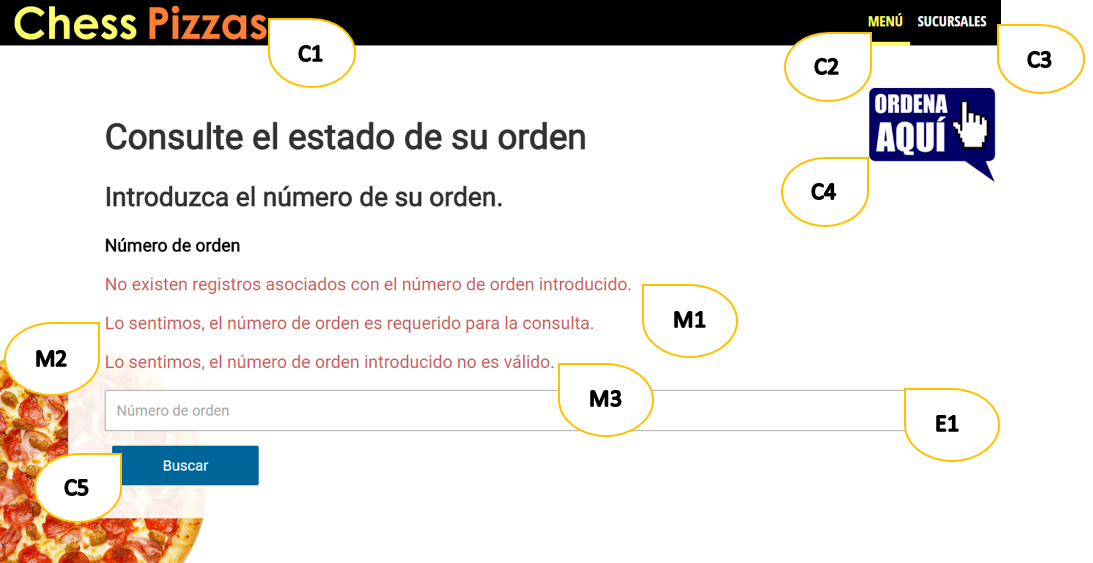
\includegraphics[width=1.1\textwidth]{images/1}
		\caption{Pantalla ''Consultar orden 1''.}
	\end{figure}
	
\subsection{Entradas:}
\begin{itemize}
\item \textbf{E1} El número de orden compuesto por 5 dígitos.
\end{itemize}

\subsection{Comandos:}
\begin{itemize}
\item \textbf{C1} Redirige al cliente a la pantalla principal del sistema.
\item \textbf{C2} Redirige al cliente a la pantalla con la información sobre las diferentes especialidades con sus respectivos precios.
\item \textbf{C3} Redirige al cliente a la pantalla con la información de las sucursales que operan dentro de México.
\item \textbf{C4} Redirige al cliente a la pantalla para realizar una nueva orden.
\item \textbf{C5} El sistema obtiene el número de orden de la entrada E1 y realiza la consulta de la orden asociada con el número de orden introducida. En caso de encontrar resultados, el sistema muestra la pantalla ''Consultar orden 2''
\end{itemize}

\subsection{Mensajes:}
\begin{itemize}
\item \textbf{M1} Se muestra cuando al haber introducido el número de orden y haber dado clic en el comando C1, el sistema no encuentra registros sobre esa orden.
\item \textbf{M2} Se muestra cuando el cliente da clic en el comando C1 sin haber introducido un número de orden en la entrada E1.
\item \textbf{M3} Se muestra cuando el cliente da clic en el comando C1 y el sistema detecta que el número introducido en la entrada E1 no tiene el formato requerido.
\end{itemize}

\section{Pantalla ''Consultar orden 2''}

Esta pantalla aparece cuando el cliente da clic en el comando C5 del  pantalla ''Consultar orden 1'' y el sistema encuentra resultados de la orden.

\begin{figure}[htbp!]
		\centering
			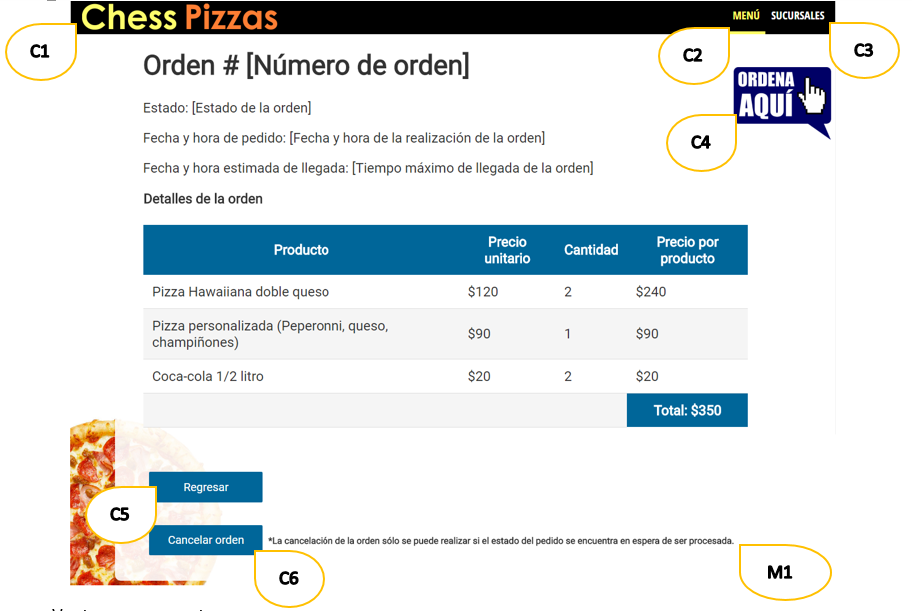
\includegraphics[width=1.1\textwidth]{images/2}
		\caption{Pantalla ''Consultar orden 2''}
	\end{figure}


\subsection{Ventanas emergentes:}
\begin{itemize}
\item \textbf{VE1} Aparece cuando el cliente da clic en el comando C6.
\begin{figure}[htbp!]
		\centering
			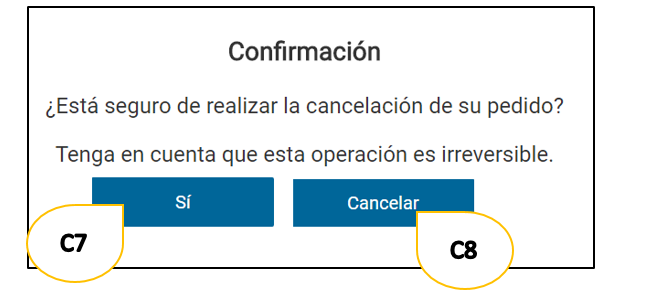
\includegraphics[width=0.8\textwidth]{images/3}
		\caption{Ventana emergente 1}
	\end{figure}
\end{itemize}


\begin{itemize}
\item \textbf{VE2} Aparece cuando el cliente oprime el comando C7 y la operación de cancelación de orden es exitosa.
\begin{figure}[htbp!]
		\centering
			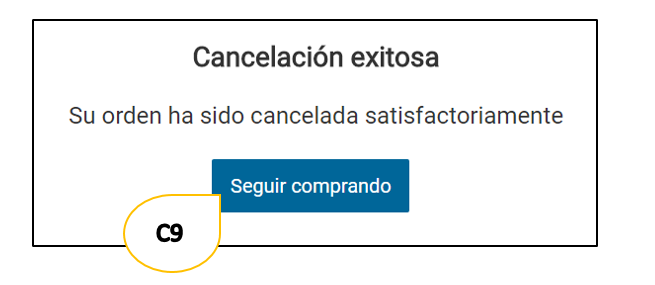
\includegraphics[width=0.8\textwidth]{images/4}
		\caption{Ventana emergente 2}
	\end{figure}
\end{itemize}
\newpage
\begin{itemize}
\item \textbf{VE3} Aparece cuando el cliente oprime el comando C7 y el estado de la orden es diferente a ''En espera de ser procesada''.
\begin{figure}[htbp!]
		\centering
			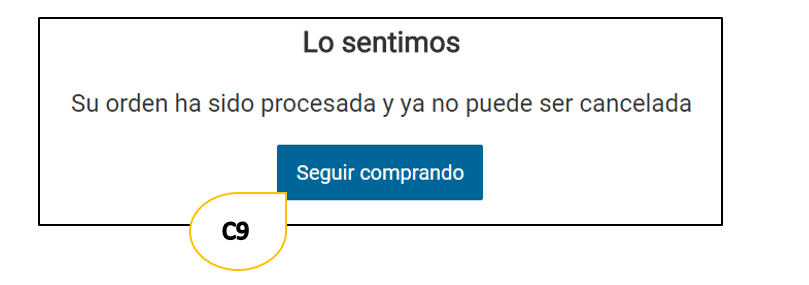
\includegraphics[width=0.8\textwidth]{images/5}
		\caption{Ventana emergente 3}
	\end{figure}
\end{itemize}

\subsection{Comandos:}
\begin{itemize}
\item \textbf{C1} Redirige al cliente a la pantalla principal del sistema.
\item \textbf{C2} Redirige al cliente a la pantalla con la información sobre las diferentes especialidades con sus respectivos precios.
\item \textbf{C3} Redirige al cliente a la pantalla con la información de las sucursales que operan dentro de México.
\item \textbf{C4} Redirige al cliente a la pantalla para realizar una nueva orden.
\item \textbf{C5} Redirige al cliente a la pantalla ''Consultar orden 1''.
\item \textbf{C6} El sistema muestra la ventana emergente VE1. Este botón sólo está habilitado cuando el estado del pedido sea ''En espera de ser procesada''. Dicho estado se presenta desde que el cliente termina de realizar el pedido hasta que la orden comienza a ser cocinada y el estado haya cambiado a ''En el horno''.
\item \textbf{C7} El sistema verifica que dicha orden tenga el estado ''En espera de ser procesada'' y cierra VE1. Si el estado es ''En espera de ser procesada'', se muestra VE2. En caso contrario, se muestra V3.
\item \textbf{C8} La operación de cancelación es cancelada, se cierra la ventana emergente VE1 y se muestra pantalla ''Consultar orden 2''.
\item \textbf{C9} Redirige al cliente a la pantalla principal del sistema.
\end{itemize}

\subsection{Mensajes:}
\begin{itemize}
\item \textbf{M1} Se muestra como información al cliente cuando el comando C6 ''Cancelar orden'' se encuentra deshabilitado debido a que el estado de la orden es diferente a ''En espera de ser procesada''.
\end{itemize}



\end{document}
